\documentclass[12pt,letterpaper]{report}
\usepackage[margin=1in]{geometry}
\usepackage{titlesec}
\usepackage{amsmath}
\usepackage{amssymb}
\usepackage[colorlinks=true,urlcolor=black,linkcolor=black]{hyperref}
\usepackage{graphicx}
\usepackage{textcomp}
% extra packages you need

\titleformat{\chapter}{\bf\huge}{\thechapter}{20pt}{\huge\vspace{-.5em}}

\begin{document}
\title{COMP	6961 Graduate Seminar Report:\\[.5em]
Characterizing Deprecated Deep Learning Python APIs: An Empirical Study in TensorFlow }
\author{Report by Rahul Patil (40166394)}
\maketitle

\begin{abstract}

The seminar report is based on the topic of Characterizing deprecated deep learning python APIs for the TensorFlow library by Nian Liu dated 15th September 2021 under the supervision of Dr. Weiyi Shang. Machine learning libraries have become significantly more accessible because of the rise of AI applications, with Python being the most prevalent programming language used to create them. Machine learning libraries are changed on a regular basis, which may deprecate current APIs, requiring developers to adjust their usages. However, updating outdated API usage is often not a top priority for developers, resulting in widespread use of deprecated APIs that expose library users to vulnerabilities. Software versioning has become a crucial part of the software development life cycle process as every new version of a software brings in improved performance, stability, better organization, and new features. A particular resource required by another software may use a specific API developed for the software, but with a particular version update, some API cannot meet the requirements of the framework which in turn causes the API to deprecate. Study conducted analyzed 20 TensorFlow releases spanning versions 1.0 to 2.3 to investigate API deprecation and its causes. TensorFlow's API version 1.0 till 2.3 provides an insight with more increase in deprecated APIs than the statistics of SLOC, APIs, with only a minor of these APIs removed till date. Researchers hope to gain insight into how TensorFlow deprecated APIs evolve, as well as help developers understand why APIs become deprecated and the consequences of not upgrading their models by deleting deprecated APIs. 

\end{abstract}

\pagenumbering{roman}
\setcounter{page}{0}

\tableofcontents

\chapter*{List of Symbols and Abbreviations}\addcontentsline{toc}{chapter}{List of Symbols and Abbreviations}

\noindent\begin{tabular}{ll}
SLOC & Source Lines of Code\\
API & Application Programming Interface\\
TF & TensorFlow\\
AI & Artificial Intelligence\\
SOTA & state-of-the-art\\
AST & Abstract Syntax Tree\\
DL & Deep Learning\\
ML & Machine Learning\\
$\cdots$ & \\
\end{tabular}


%%%%%%%%%%%%%%%%%%%%%%%%%%%%%%
\listoffigures\addcontentsline{toc}{chapter}{List of Figures}


%%%%%%%%%%%%%%%%%%%%%%%%%%%%%%
\listoftables\addcontentsline{toc}{chapter}{List of Tables}

%%%%%%%%%%%%%%%%%%%%%%%%%%%%%%
\chapter{Introduction}
\pagenumbering{arabic}

\section{Background on Problem Domain}

The thesis conducted here is an empirical study on deprecated Python APIs in TensorFlow, which explores findings on TF releases to investigate API deprecation and it's causes. Thus, a background overview of TensorFlow python APIs, deep learning with TF and API deprecation is essential for analysis of the problem domain.

``Section~\ref{sec:problemstatement}.'' provides brief overview of the problem statement and the research questions which facilitate the thesis. Further ``Section~\ref{sec:methodology}.'' introduces the techniques used to analyse data and retrieve results, make comparisons and the metrics used for deference between accuracy of models impacted by API deprecation.

\section{Problem Statement} \label{sec:problemstatement}

As TensorFlow advances, new Python APIs are introduced, while others may be deprecated. Although the features of deprecated APIs in common software frameworks such as Android have been extensively studied in recent years, little attention has been devoted to how TensorFlow deprecated APIs develop and the impact this has on deep learning. 

Current problem domain for APIs focuses on areas of research which provide concise idea on how many APIs are deprecated over time, which in current context is based on TensorFlow library. Why have these APIs become deprecated and their impact in real projects? To what extent are these deprecated APIs used in these projects? Do these deprecated APIs affect the accuracy of deep learning models? And to what extent does this accuracy for the deep learning models change? 

An empirical analysis of TensorFlow deprecated APIs gives developers a better understanding of how TensorFlow deprecated APIs evolve, as well as why APIs become deprecated and the consequences of not upgrading their models by deleting obsolete APIs.

\section{Methodology} \label{sec:methodology}
The overall approach involves taking note of API deprecation and it's causes for TensorFlow releases spanning from 1.0 to 2.3. The experimental setup accounts data from 20 TensorFlow releases and 12 Deep Learning models for which the data was extracted from official GitHub repository.

To get accurate statistics for the total deprecations spanning all releases, an AST was used to parse the entire TensorFlow library to keep track of API name, related annotations for deprecated APIs. Every single method or classes within these TensorFlow versions with the decorator @deprecated was added to the list of deprecated APIs and used for further analysis for the research. Information gained from the above method can be used to find SLOC, Important dates, if API was deprecated in previous versions and removed in current one denoting the survival time of an API, etc \cite{charsDeep}.

As TensorFlow is used for training deep learning models and API deprecation with it could affect accuracy of the models. To analyse the same and calculate the resultant change the deprecated APIs were manually upgraded in order check overall impact before and after updating them. There are a few statistical measures which are considered for comparison of the results which are p-value, Cohen's D and t-test in order to compare model accuracy before and after deprecated API modifications in this study.

The p-value is a statistical indicator of the statistical significance of links between two groups of data. It is a probability that indicates whether the null hypothesis (i.e., that there is no difference between the two groups of data samples) is rejected. The null hypothesis is rejected if the p-value is less than a particular threshold (usually 0.05), implying that there is a difference between the two data samples. 

Cohen's D is a measure of the magnitude of the difference between two groups of data. The association between two data groups becomes stronger as the effect size develops. Cohen's D of 0.2 indicates a moderate influence, 0.5 indicates a medium effect, and 0.8 indicates a high effect. Cohen's D is unaffected by sample size, but the p-value is, and with a sufficiently big sample, the p-value will nearly always be significant. 

The t-test is a statistical test that is used to compare two groups' means. Independent samples and paired samples are used in a two-sample t-test. Independent samples are unrelated to one another, whereas paired samples are related to one another. Two independent samples of model accuracies before and after deprecated API modifications. As a result, Independent t-test used used to compare the model accuracy before and after upgrading the deprecated APIs in our experiment.

\section{Assumptions and Limitations} \label{sec:assumptions}

The empirical study done for the thesis compares API deprecation of TensorFlow library, which is a free and open-source software library for machine learning and artificial intelligence with the API deprecation in Android, which is a full-fledged mobile operating system. As TensorFlow is generally used for deep learning and Android is like a modified version of the Linux kernel, both have different user base, usage scenarios, dependencies, implementation, abstraction layers, frameworks, requirements etc.

The comparison is limited to two different systems, wherein a comparison between two AI libraries like PyTorch and TensorFlow could have had added a close relation between systems designed for similar work.

%%%%%%%%%%%%%%%%%%%%%%%%%%%%%%
\chapter{Background}

The research work being concluded here requires firm knowledge for a few background terms like the TensorFlow library, What is API and API deprecation in the context of a library like TF and Deep Learning Models in AI.

``Section~\ref{sec:tensorflow}.'' provides brief overview about the TF library developed by the Google brain team \cite{GoogleBrain,DLwithTensor}. Further ``Section~\ref{sec:apidep}.'' introduces the formal definition of API deprecation and how it's handled in TF. Section concludes with ``Section~\ref{sec:deeplearning}.'', which gives brief overview about deep learning and it's use in AI.

\section{TensorFlow} \label{sec:tensorflow}
TensorFlow is a machine learning and artificial intelligence software library that is free and open source. It can be used for a variety of applications, but it focuses on deep neural network training and inference.

TensorFlow is a large-scale machine learning system that works in a variety of contexts. Its computational paradigm is built on mutable state dataflow graphs. Graph nodes can be assigned to multiple computers in a cluster, as well as CPUs, GPUs, and other devices inside each system. TensorFlow may be used for several tasks, but it's best known for deep neural network training and inference. It is used as a research and deployment platform for machine learning systems in a variety of fields, including speech recognition, computer vision, robotics, information retrieval, and natural language processing\cite{tensorflowScale}.

\begin{figure}[h]
    \begin{center}
    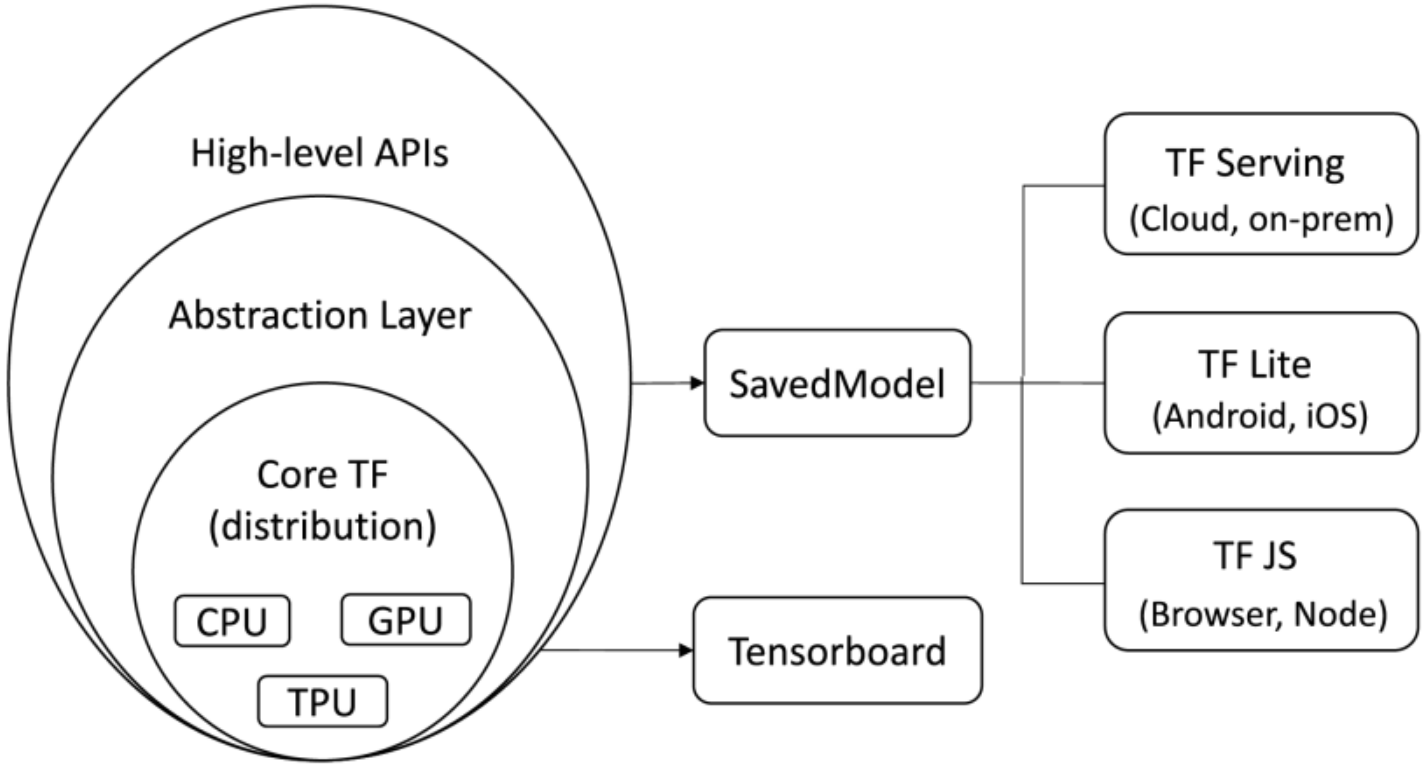
\includegraphics[width=0.5\linewidth]{comp6961-report-framework.png}
    \end{center}
       \caption{TensorFlow Framework\cite{apiEvo}\label{framework}}
\end{figure}

TensorFlow is a popular deep learning framework with a few APIs to assist users in creating deep learning applications. Core TensorFlow allows for distributed execution across numerous devices (e.g., CPUs, GPUs and TPUs). The abstract layer, which offers components for users to design neural network models and establish metrics and losses for model assessment, is the following layer. The third layer offers high-level APIs, such as keras and estimator, that let users to easily build and train models as can be seen in Figure~\ref{framework}. TensorFlow now standardises the Saved Model, which may execute on several runtimes, including cloud, web browsers, and mobile devices, where there is a model.

TensorFlow is made up of several abstraction layers. The top layer contains object-oriented APIs at a high level. The components for generating bespoke models make up the second layer from the top. The third layer is a Python-based low-level API as infered from Figure~\ref{layers}.
These APIs can be used to construct and implement new machine learning algorithms by developers. The TensorFlow kernel API, which is written in C++, is the fourth layer. Finally, the hardware layer is where TensorFlow code may execute on a variety of platforms, including CPU, GPU, and TPU  \cite{apiEvo}.

\begin{figure}[h]
    \begin{center}
    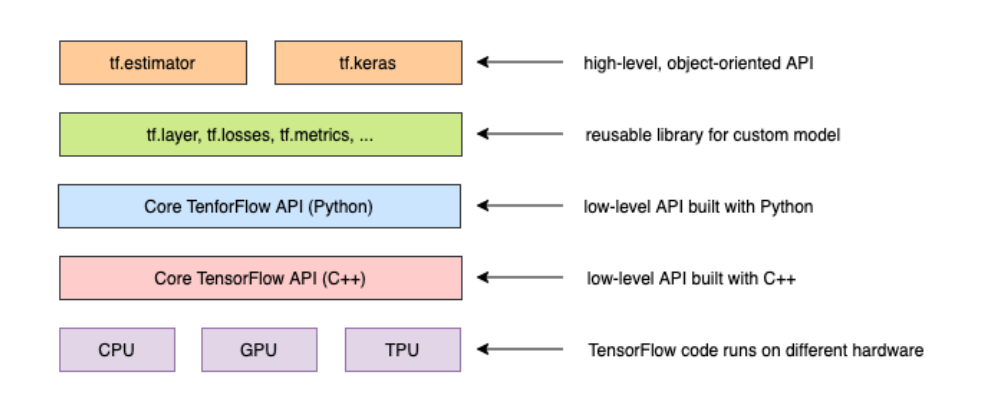
\includegraphics[width=0.8 \linewidth]{comp6961-report-hierarchy.png}
    \end{center}
       \caption{Layers of TensorFlow API\cite{charsDeep}\label{layers}}
\end{figure}

\section{API deprecation} \label{sec:apidep}

The objective of an API is to make programming easier by abstracting the underlying functionality and only exposing the objects or actions that the developer need.
An application programming interface (API) is a link between two computers or applications. It's a form of software interface that provides a service to other programs. An API specification is a document or standard that explains how to create or utilise a connection or interface. Interfaces are bound to change as per usage and updates to the end point applications with change in features. 

Due to changes in the API, a deprecated API is one that should no longer be used. While deprecated classes, methods, and fields are still implemented, they may be deleted in future versions, therefore they should be avoided in new code and, if feasible, modify existing code to avoid using them. With the introduction of new TensorFlow versions, some APIs are unable to match the framework's requirements, resulting in API deprecation.

\begin{table}[h]
    \begin{center}
    \begin{tabular}{|l|c|c|c|}
    \hline
         TF Version & SLOC & APIs & Deprecated APIs \\
    \hline\hline 
    2.3 & 412K & 6,586 & 190 \\
    2.2 & 386K & 6,251 & 166 \\
    2.1 & 355K & 5,934 & 190 \\
    2.0 & 337K & 5,714 & 155 \\
    1.15 & 338K & 5,707 & 150 \\
    1.14 & 314K & 5,338 & 150 \\
    1.13 & 257K & 4,419 & 116 \\
    1.12 & 229K & 3,786 & 45 \\
    1.11 & 211K & 3,470 & 29 \\
    1.10 & 206K & 3,357 & 23 \\
    1.9 & 195K & 3,251 & 22 \\
    1.8 & 188K & 3,172 & 22 \\
    1.7 & 182K & 3,033 & 22 \\
    1.6 & 176K & 2,948 & 22 \\
    1.5 & 167K & 2,798 & 21 \\
    1.4 & 154K & 2,612 & 15 \\
    1.3 & 113K & 2,002 & 15 \\
    1.2 & 106K & 1,888 & 13 \\
    1.1 & 90K & 1,659 & 13 \\
    1.0 & 82K & 1,525 & 13 \\
    \hline
    \end{tabular}
    \end{center}
    \caption{Overview of TensorFlow versions with deprecated APIs.\label{versionsDep}}
 \end{table}

With TensorFlow, These APIs are marked as deprecated using Python annotations, and then deleted after a reasonable period (e.g., several releases of the framework).
Developers can use the deprecated() decorator (i.e., @deprecated) to indicate deprecated APIs. The arguments supplied to deprecated() in this decorator can be used to show a deprecation message, which tells users that an API is deprecated, when it will be removed, and what developers can do in the meanwhile. Table~\ref{versionsDep} shows the number of deprectaed APIs over the period of TF version releases.  

\section{Deep Learning : Deep Dive} \label{sec:deeplearning}
Deep learning is a branch of machine learning that employs artificial neural networks with structures and functions inspired by the human brain. Despite being a relatively new method, it has recently gained a lot of popularity. In many situations where machine learning has been effective at certain rates, deep learning has had a substantially greater success rate. It is especially useful for classifying large data sets since it produces quick and accurate results.

It has been widely used in AI domains, such as image classification, object detection, pattern recognition, and natural language processing (NLP), and proven to be successful.

\begin{figure}[h]
    \begin{center}
    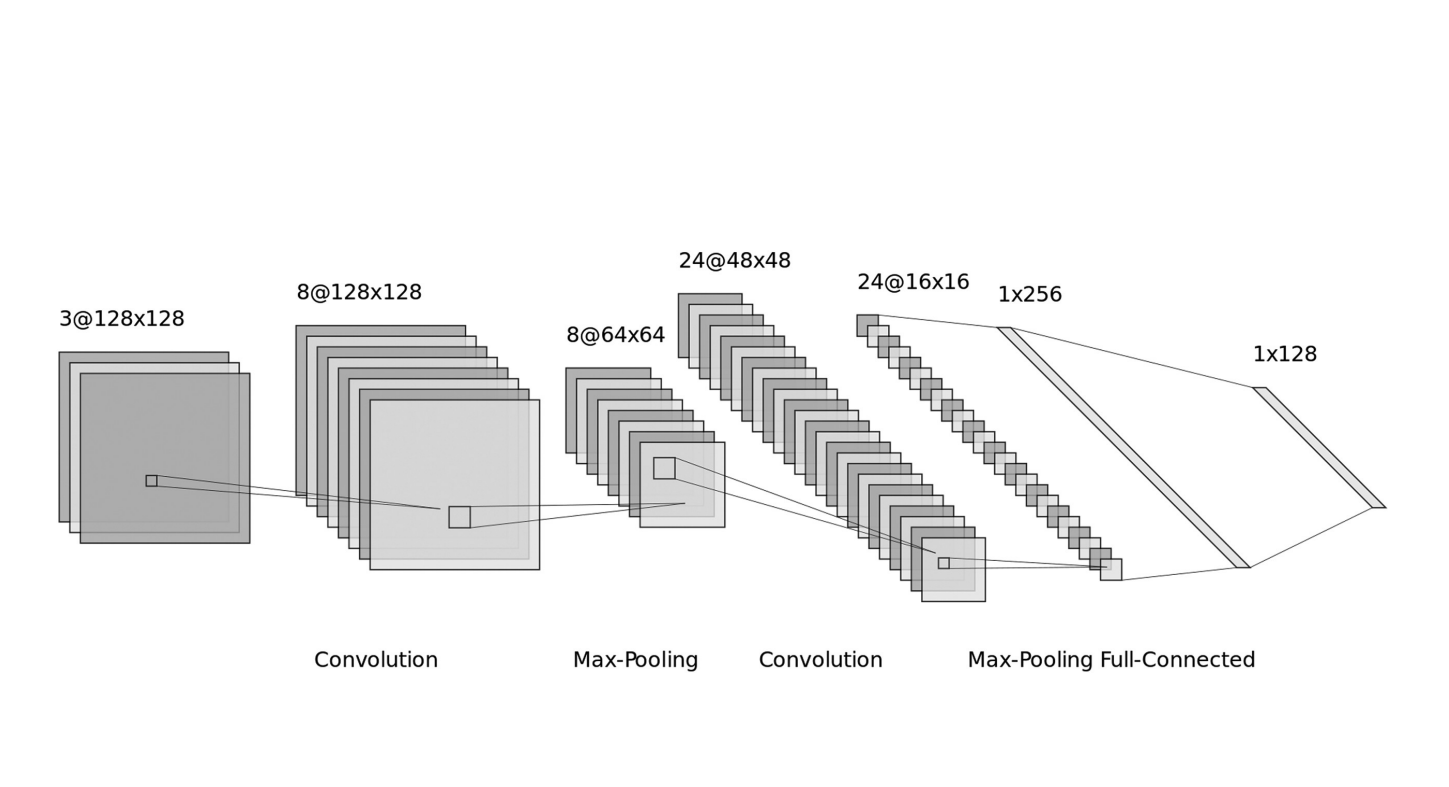
\includegraphics[width=0.5\linewidth]{comp6961-report-cnn.png}
    \end{center}
       \caption{A Deep Convolution Neural Network\cite{DLwithTensor}\label{cnn}}
\end{figure}


While traditional machine learning algorithms assume classification methods to be either 0 or 1, deep learning may produce numerical results in the range of 0 to 1. As a result, more precise answers to the present problem may be provided, and classification systems can attain faster and higher accuracy levels \cite{dlEvo}. A model class may be generated using a CNN in deep learning to enable powerful and frequently correct assumptions by adjusting various parameters. In deep learning investigations, a variety of libraries are employed. To train and evaluate deep learning CNN models, each input picture will be passed through a sequence of convolution layers using filters (Kernals), Pooling, fully connected layers (FC), and the Softmax function to categorise an item with probabilistic values ranging from 0 to 1. The Figure~\ref{cnn} depicts the whole CNN workflow for processing an input picture and classifying objects based on values. The first layer to extract features from an input picture is convolution. By learning visual attributes with tiny squares of input data, convolution retains the link between pixels. When the photos are too huge, the pooling layers portion would lower the number of parameters. Spatial pooling, also known as subsampling or downsampling, decreases the dimensionality of each map while preserving crucial data. Finally classifies pictures with the use of an activation function.

%%%%%%%%%%%%%%%%%%%%%%%%%%%%%%
\chapter{Technical Contributions}

\section{TensorFlow API deprecation and the Why?} \label{sec:deprecationwhy}
The empirical study conducted here provides AI researchers a concise data depicting the total TensorFlow APIs deprecated spanning from version from 1.0 to 2.3 investigating the status of API deprecation in TensorFlow could also help developers better understand the evolution patterns of TensorFlow and prepare for the migration of the deprecated APIs in their projects. The research also provides and outlines reasons for this API deprecation.

Analysis involves examination of 20 TensorFlow branches with AST used for static analysis of the TensorFlow library code. As mentioned in ``Section~\ref{sec:methodology}.'' deprecated APIs in TensorFlow are identified by the decorator @deprecated. Thus, if a class or method had such a decorator, it was considered deprecated and added to a list. Furthermore, if an API was deprecated in the previous version and disappeared in the current version, it was removed; if an API was not deprecated in the previous version but becomes deprecated in the current version, we consider it newly deprecated.

With the evolution of TensorFlow data analysis resulted with the following as the number of SLOCs, APIs, and Deprecated APIs grows, with Deprecated APIs growing even faster. SLOC has grown five-fold from TensorFlow 1.0 to TensorFlow 2.3, whereas the number of APIs has increased four-fold. The number of APIs that have been deprecated has risen from 13 to 190. (i.e., nearly 15 times). Further unveiling that As TensorFlow progresses, the number of deprecated APIs grows, with a considerable rise in TensorFlow 1.13. Only a tiny percentage of deprecated APIs (4.52 percent) are finally deleted, yet their lifespan is rather short (2 versions in median). Since their introduction into TensorFlow, most deprecated APIs have taken a lengthy time to become deprecated (12 versions on average).

\begin{table}[h]
    \begin{center}
    \begin{tabular}{|l|c|c|}
    \hline
          & Deprecation Rationale & Level \\
    \hline\hline

    1 & API Optimization & Method \\
    2 & API Name Change & Method \\
    3 & Compatibility Issue & Method \\
    4 & Feature Deleting  & Method \\
    5 & Parameter Name Change & Parameter \\
    6 & Unnecessary Parameter & Parameter \\
    \hline
    \end{tabular}
    \end{center}
    \caption{API deprecation rationales.\label{api_deprecation}}
 \end{table}

This brings the research forward to the major reasons for the API deprecation and its impacts.
The former methodology used AST to keep track of the total deprecated APIs, along with that further exploring the deprecation message extracted by AST was used to discover rationales of API deprecation. Source code was analysed if in case deprecation message was missing which resulted with deprecation rationales as shown in Table~\ref{api_deprecation}.

Deprecations of TensorFlow API methods are driven by optimization improvements (e.g., API Optimization (53.77\%), whereas parameter deprecations are driven by usability improvements (e.g., Parameter Name Change (91.67\%) \cite{charsDeep}.

\section{Usage of TF deprecated APIs} \label{sec:tfdepapi}
It is imperative for AI researchers and developers to know about the rationale behind API deprecation and change to its usage.  Methodology provided in ``Section~\ref{sec:methodology}.'' also covers the deep learning models maintained by official TensorFlow GitHub organization.
Deprecated APIs frequently go through a deprecated-replace-remove cycle, in which APIs are initially identified as deprecated, and then replacement notifications are sent to developers to help with code migration.

\begin{table}[h]
    \begin{center}
    \begin{tabular}{|l|c|c|c|c|}
    \hline
         Branch & SLOC & Methods & Models & API Version \\
    \hline\hline 
    r2.3 & 53K & 939 & 12 & 2.3 \\
    r2.2 & 51K & 956 & 9 & 2.2 \\
    r2.1 & 47K & 848 & 9 & 2.1 \\
    r2.0 & 31K & 638 & 8 & 2.0 \\
    r1.13 & 12K & 285 & 5 & 1.13 \\
    r1.12 & 11K & 254 & 5 & 1.12 \\
    r1.11 & 10K & 227 & 5 & 1.11 \\
    r1.10 & 9K & 218 & 5 & 1.10 \\
    \hline
    \end{tabular}
    \end{center}
    \caption{Overview of selected Models branches.\label{model_overview}}
 \end{table}

The amount of source lines of code (SLOC) has risen by six times from branch r1.10 (the earliest branch) to branch r2.3 (the most current branch at the time of the research), while the number of methods has increased by more than four times. In addition, the repository now includes a total of 12 deep learning models, up from five previously as shown in Table~\ref{model_overview}.

The findings after the overall analysis jots down to the fact that TensorFlow formally maintains Models, it still has deprecated APIs. Prior to TensorFlow 1.13, there was no deprecated API in Models. However, since the release of TensorFlow 1.13, deprecated APIs have appeared (5-10\% of TensorFlow deprecated APIs), which could be ascribed to TensorFlow 1.13's considerable increase in deprecated APIs. 

\newpage

\section{Consequences and Results} \label{sec:consequences}
A major impact of deprecated APIs can be seen in real world projects which were already build and are currently being validated on real world data. Thus, many such deep learning projects may suffer change with usage of APIs which will be deprecated or removed. As a result, getting to know about the variability of the change in model workflow and model accuracy is significant to many AI researchers. To study the potential influence of deprecated APIs on deep learning models, manually upgrading the deprecated APIs detected in earlier phase and comparing the model accuracy difference before and after updating it would provide accurate change in model accuracy values.

There can be several deprecated APIs used in TF Models which have no impact on model accuracy and thus were excluded from the overall experiment, as these are related to displaying GPU info, iterators, etc. While the rest of the Models were considered for the experiment. As a result the necessary deep learning models were trained and tested which were important for model computation. The overall experiments didn't show any significant changes. As introduced in ``Section~\ref{sec:methodology}.'', The null hypothesis is that model accuracy remains constant before and after deprecated API updates; hence, if the p-value is less than the threshold (0.05), the model accuracy differs; otherwise, it does not. The metrics were calculated for the trained and tested deep learning models for the 12 deprecated APIs and resulted with none of the APIs with a p-value lower than the threshold (0.05). For six tests, Cohen's D shows a medium effect and for seven tests, a minor effect. As a result, consumers of these APIs are not enticed to move to the replacement APIs due to changes in accuracy.

%%%%%%%%%%%%%%%%%%%%%%%%%%%%%%
\chapter{Conclusions and Impact}

    The empirical study done here looked at the evolution of deprecated APIs throughout 20 TensorFlow versions, from TensorFlow 1.0 to TensorFlow 2.3, along with rationale behind these API deprecations. Analysis of deep learning models to investigate the influence of deprecated APIs on model accuracy was done, which would help AI researchers to better understand how TensorFlow deprecated APIs evolve, as well as the consequences of not upgrading their models. Thesis does compare the extent API deprecation of TensorFlow with Android and rationale behind deprecation with the one in Java which is useful, but a precise comparison with a deep learning or machine learning library like PyTorch could have had provided AI researchers to closely follow the statistics as they fall on similar usage scenarios. The study concludes that 1) the number of deprecated APIs grows steadily as TensorFlow advances, and that while only a tiny percentage (4.52\%) of deprecated APIs are finally deleted, their survival duration is very short (2 versions in median). Since their introduction into TensorFlow, most deprecated APIs have taken a lot of time to become deprecated (12 versions on average as per results from analysis). 2) Optimization improvements (e.g., API Optimization (53.77 percent) for the method level and usability improvements (e.g., Parameter Name Change (91.67 percent) for the parameter level are the key reasons for deprecating TensorFlow API. 3) In Models projects, there are just a few deprecated APIs (5-10\%). 4) None of the deprecated APIs we looked at have a p-value less than 0.05, and Cohen's D shows a medium impact for six tests and a minor effect for seven. As a result, there is no discernible change in accuracy following deprecated API upgrades. Future work on API deprecation might be aided by preliminary comparisons with similar deep learning libraries such as PyTorch, Theano, and others, as well as the gathering of additional deep learning projects to assess the influence of deprecated APIs on model performance.


%%%%%%%%%%%%%%%%%%%%%%%%%%%%%%
\begin{thebibliography}{9}
    \addcontentsline{toc}{chapter}{Bibliography}

    \bibitem{tensorflowScale}
    Martín Abadi. 2016.
    \textit{ "TensorFlow: learning functions at scale. In Proceedings of the 21st ACM SIGPLAN International Conference on Functional Programming (ICFP 2016)." Association for Computing Machinery, New York, NY, USA, 1. DOI:https://doi.org/10.1145/2951913.2976746}
    
    \bibitem{apiEvo}
    Z. Zhang, Y. Yang, X. Xia, D. Lo, X. Ren and J. Grundy
    \textit{"Unveiling the Mystery of API Evolution in Deep Learning Frameworks: A Case Study of Tensorflow 2," 2021 IEEE/ACM 43rd International Conference on Software Engineering: Software Engineering in Practice (ICSE-SEIP), 2021, pp. 238-247, doi: 10.1109/ICSE-SEIP52600.2021.00033.}
    
    \bibitem{charsDeep}    
    Liu, N. 2021.
    \textit{"Characterizing Deprecated Deep Learning Python APIs: An Empirical Study on TensorFlow" - Spectrum: Concordia University Research Repository. [Accessed 8 December 2021].}

    \bibitem{DLwithTensor}
    Pang, Bo, et al.
    \textit{“Deep Learning With TensorFlow: A Review.” 
    Journal of Educational and Behavioral Statistics, vol. 45, no. 2, 
    Apr. 2020, pp. 227–248, doi:10.3102/1076998619872761.}

    \bibitem{GoogleBrain}
    Mallory Helms, Shaun V. Ault, Guifen Mao, and Jin Wang. 2018.
    \textit{"An Overview of Google Brain and Its Applications." In Proceedings of the 2018 International Conference on Big Data and Education (ICBDE '18). Association for Computing Machinery, New York, NY, USA, 72–75. DOI:https://doi.org/10.1145/3206157.3206175}
    
    \bibitem{tensorFlow}
    Goldsborough, P., 2016.
    \textit{"A Tour of TensorFlow." [online] arXiv.org. Available at: https://arxiv.org/abs/1610.01178 [Accessed 10 December 2021].}
    
    \bibitem{dlEvo}
    F. Ertam and G. Aydın
    \textit{"Data classification with deep learning using Tensorflow," 2017 International Conference on Computer Science and Engineering (UBMK), 2017, pp. 755-758, doi: 10.1109/UBMK.2017.8093521.}
    
\end{thebibliography}

\end{document}
